\documentclass{beamer}
\usepackage{tikz}
\usepackage{tikzsymbols}
\usepackage{pgfplots}
\usetikzlibrary{patterns}
\usepackage{scalerel}
\usepackage{multicol}
\usepackage{caption}
\usepackage{subcaption}
\usepackage{graphicx}
\usepackage{xcolor}
\usepackage{mathtools}
\usetikzlibrary{patterns.meta}
\usetikzlibrary{arrows.meta}
\usepackage{hyperref}
\usetikzlibrary{backgrounds}
\usepackage{amsmath}
\usetheme{Boadilla}

\pgfplotsset{compat=1.11,
                /pgfplots/ybar legend/.style={
                /pgfplots/legend image code/.code={%
                \draw[##1,/tikz/.cd,yshift=-0.25em]
                    (0cm,0cm) rectangle (3pt,0.8em);},
                },
}

\newcommand{\nodesize}{.7cm}

%Information to be included in the title page:
\title{\texttt{BisPy}}
\subtitle{un pacchetto Python per il calcolo\\ della massima bisimulazione di grafi diretti}

\author{Francesco Andreuzzi}
\institute{Università degli Studi di Trieste,\\Dipartimento di Ingegneria e Architettura}
\date{8 Luglio 2021}

\makeatletter
\setbeamertemplate{footline}
{
  \leavevmode%
  \hbox{%
  \begin{beamercolorbox}[wd=.333333\paperwidth,ht=2.25ex,dp=1ex,center]{author in head/foot}%
    \usebeamerfont{author in head/foot}\insertshortauthor%~~\beamer@ifempty{\insertshortinstitute}{}{(\insertshortinstitute)}
  \end{beamercolorbox}%
  \begin{beamercolorbox}[wd=.333333\paperwidth,ht=2.25ex,dp=1ex,center]{title in head/foot}%
    \usebeamerfont{title in head/foot}\insertshorttitle
  \end{beamercolorbox}%
  \begin{beamercolorbox}[wd=.333333\paperwidth,ht=2.25ex,dp=1ex,right]{date in head/foot}%
    \usebeamerfont{date in head/foot}\insertshortdate{}\hspace*{2em}
    \insertframenumber{} / \inserttotalframenumber\hspace*{2ex}
  \end{beamercolorbox}}%
  \vskip0pt%
}
\makeatother

\begin{document}
\beamertemplatenavigationsymbolsempty

{\usebackgroundtemplate{%
    \parbox[c][\paperheight][c]{\paperwidth}{\centering \tikz\node[opacity=0.08] {\includegraphics[width=8cm,height=8cm]{../imgs/logo.png}};}}
    \begin{frame}
        \maketitle
        {\scriptsize Anno accademico 2020-2021 \hfill Relatore: Prof. Alberto Casagrande}
    \end{frame}
}

\begin{frame}\frametitle{Grafi orientati, terminologia}
    \begin{gather*}
        V = \{a,b,c,d,e\}\\
        E = \{\langle a,b\rangle, \langle b,c\rangle, \langle a,d\rangle, \langle c,e\rangle, \langle d,e\rangle\}
    \end{gather*}

    \begin{figure}[t]
        \centering
        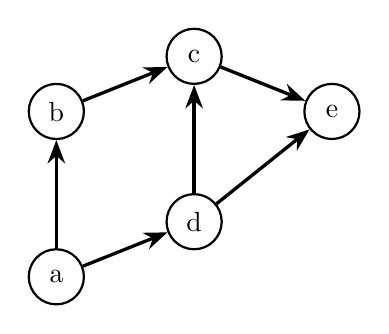
\begin{tikzpicture}[scale=0.7]
            \begin{scope}[every node/.style={circle,thick,draw,minimum size=\nodesize}]
                \node (a) at (0,0) {a};
                \node (b) at (0,3) {b};
                \node (c) at (2.5,4) {c};
                \node (d) at (2.5,1) {d};
                \node (e) at (5,3) {e};
            \end{scope}

            \begin{scope}[>={Stealth[black]},,
                every edge/.style={draw=black,very thick}]
                \path [->] (a) edge node {} (b);
                \path [->] (b) edge node {} (c);
                \path [->] (a) edge node {} (d);
                \path [->] (d) edge node {} (c);
                \path [->] (d) edge node {} (e);
                \path [->] (c) edge node {} (e);
            \end{scope}
            \end{tikzpicture}
    \end{figure}

    \bigskip

    \begin{block}{Definizione}
        Se $\langle a,b \rangle \in E \implies b$ è un nodo \emph{figlio} di $a$.\\
        Un nodo privo di figli è detto \emph{pozzo}.
    \end{block}
\end{frame}

\begin{frame}\frametitle{Bisimulazione}
    \begin{block}{Definizione: Bisimulazione $\mathcal{B} \subseteq V \times V$}
        \centering
        Se $(a,b) \in \mathcal{B}$, allora da $a$ è possibile spostarsi verso un nodo \emph{figlio} di $a$ che sia in relazione con un nodo \emph{figlio} di $b$, e viceversa.
    \end{block}

    \bigskip

    \begin{figure}
        \begin{subfigure}{0.55\textwidth}
            \centering
            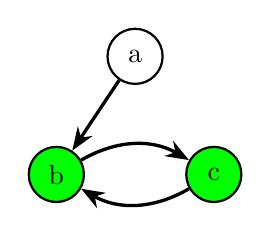
\begin{tikzpicture}[scale=0.5]
                \begin{scope}[every node/.style={circle,thick,draw,minimum size=\nodesize}]
                    \node (a) at (0,6) {a};
                    \node[fill=green] (c) at (2,3) {c};
                    \node[fill=green] (b) at (-2,3) {b};
                \end{scope}

                \begin{scope}[>={Stealth[black]},
                    every edge/.style={draw=black,very thick}]
                    \path [->] (a) edge node {} (b);

                    \path [->] (b) edge [bend left] node {} (c);
                    \path [->] (c) edge [bend left] node {} (b);
                \end{scope}
            \end{tikzpicture}
        \end{subfigure}
        \hfill
        \begin{subfigure}{0.44\textwidth}
            \Large
            \begin{gather*}
                \mathcal{B} = \{(b,c)\}
            \end{gather*}
        \end{subfigure}
    \end{figure}

    \begin{block}{Definizione: Nodi bisimili}
        \centering
        I nodi $a,b$ sono \emph{bisimili} se esiste una bisimulazione $\mathcal{B}$ tale che $(a,b) \in \mathcal{B}$.
    \end{block}
\end{frame}

\begin{frame}\frametitle{Massima bisimulazione}
    \begin{block}{Definizione}
        La \emph{massima bisimulazione} su $G = (V,E)$ è la bisimulazione $\mathcal{B}_\mathcal{M}$ tale che:
        \begin{gather*}
            \mathcal{R} \subseteq \mathcal{B}_\mathcal{M} \quad \text{ per ogni bisimulazione } \mathcal{R} \text{ su } G.
        \end{gather*}
    \end{block}

    \bigskip\bigskip

    Si può dimostrare che:
    \begin{enumerate}
        \item La \emph{massima bisimulazione} è \textbf{unica};
        \item La \emph{massima bisimulazione} è una \emph{relazione di equivalenza}

        $\implies$ induce un partizionamento su $V$;
        \item $\displaystyle \mathcal{B}_\mathcal{M}(a,b) \,\,\,\equiv \bigcup_{\substack{\mathcal{R} \text{ è una}\\\text{bisimulazione}}} \mathcal{R}$;
        \item $\mathcal{B}_\mathcal{M}$ definita come nel punto 3. è una \emph{bisimulazione}.
    \end{enumerate}
\end{frame}

\begin{frame}\frametitle{Massima bisimulazione -{}- {\normalsize Esempio e applicazioni pratiche}}
    \begin{figure}
        \begin{subfigure}{0.35\textwidth}
            \centering
            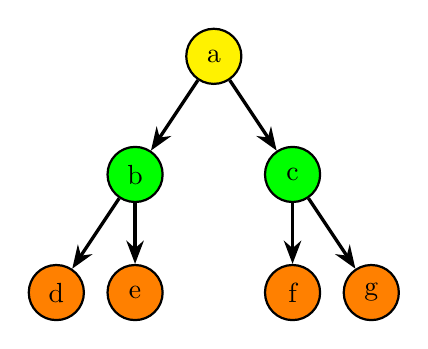
\begin{tikzpicture}[scale=0.5]
                \begin{scope}[every node/.style={circle,thick,draw,minimum size=\nodesize}]
                    \node[fill=yellow] (a) at (0,6) {a};
                    \node[fill=green] (c) at (2,3) {c};
                    \node[fill=green] (b) at (-2,3) {b};
                    \node[fill=orange] (d) at (-4,0) {d};
                    \node[fill=orange] (e) at (-2,0) {e};
                    \node[fill=orange] (f) at (2,0) {f};
                    \node[fill=orange] (g) at (4,0) {g};
                \end{scope}

                \begin{scope}[>={Stealth[black]},
                    every edge/.style={draw=black,very thick}]
                    \path [->] (a) edge node {} (b);
                    \path [->] (a) edge node {} (c);

                    \path [->] (b) edge node {} (d);
                    \path [->] (b) edge node {} (e);

                    \path [->] (c) edge node {} (f);
                    \path [->] (c) edge node {} (g);
                \end{scope}
            \end{tikzpicture}
        \end{subfigure}
        \begin{subfigure}{0.45\textwidth}
            \scriptsize
            \begin{align*}
                \mathcal{B}_\mathcal{M} = \big\{&\colorbox{yellow}{$(a,a)$}, \colorbox{green}{$(b,c), (c,b)$},\\
                &\colorbox{green}{$(b,b), (c,c)$}, \colorbox{orange}{$(d,d)$},\\
                &\colorbox{orange}{$(e,e), (f,f), (g,g)$},\\
                &\colorbox{orange}{$(d,e), (e,d), (d,f)$},\\
                &\colorbox{orange}{$(f,d), (d,g), (g,d)$},\\
                &\colorbox{orange}{$(e,f), (f,e), (e,g)$},\\
                &\colorbox{orange}{$(g,e), (f,g), (g,f)$}\big\}
            \end{align*}
        \end{subfigure}
        \begin{subfigure}{0.1\textwidth}
            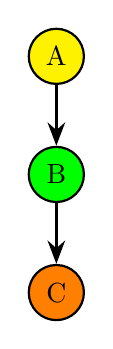
\begin{tikzpicture}[scale=0.5]
                \begin{scope}[every node/.style={circle,thick,draw,minimum size=\nodesize}]
                    \node[fill=yellow] (A) at (0,6) {A};
                    \node[fill=green] (B) at (0,3) {B};
                    \node[fill=orange] (C) at (0,0) {C};
                \end{scope}

                \begin{scope}[>={Stealth[black]},
                    every edge/.style={draw=black,very thick}]
                    \path [->] (A) edge node {} (B);
                    \path [->] (B) edge node {} (C);
                \end{scope}
            \end{tikzpicture}
        \end{subfigure}
    \end{figure}

    \bigskip

    \begin{multicols}{2}
        \begin{itemize}
            \item Ricerca di nodi equivalenti;
            \item Minimizzazione;
            \item Concurrency theory;
            \item XML indexing.
        \end{itemize}
    \end{multicols}
\end{frame}

\begin{frame}\frametitle{Algoritmi per il calcolo della massima bisimulazione}
    \textbf{Non incrementali}, complessità asintotica $|E| \log |V|$
    \begin{itemize}
        \item Algoritmo di Paige-Tarjan;
        \item Algoritmo di Dovier-Piazza-Policriti;

        \qquad $\mathcal{B}_\mathcal{M}(u,v) \implies$ \texttt{rank}$(u) =$ \texttt{rank}$(v)$.
    \end{itemize}

    \bigskip

    \textbf{Incrementali}
    \begin{itemize}
        \item Algoritmo incrementale di Saha.
    \end{itemize}
\end{frame}

\begin{frame}[fragile]\frametitle{BisPy}
    \begin{itemize}
        \item Python 3;
        \item Open source (\url{https://github.com/fAndreuzzi/BisPy});
        \item Testato su diverse tipologie di grafo, di dimensioni varie.
    \end{itemize}

    \begin{example}
        \begin{verbatim}
        from bispy import paige_tarjan

        # creazione del grafo
        graph = networkx.balanced_tree(2,3)

        # calcolo della massima bisimulazione
        paige_tarjan(graph)

        >>> [(7, 8, 9, 10, 11, 12, 13, 14), (3, 4, 5, 6),
            (1, 2), (0,)]
        \end{verbatim}
    \end{example}
\end{frame}

\begin{frame}\frametitle{Risultati sperimentali I -{}- {\normalsize Paige-Tarjan, Dovier-Piazza-Policriti}}
    \begin{figure}[b!]
        \centering
        \captionsetup[subfigure]{labelformat=empty}
        \begin{subfigure}{0.49\textwidth}
            \begin{tikzpicture}
                \begin{axis}[
                    axis on top,
                    width=\textwidth,
                    ytick style={draw=none},
                    xtick style={draw=none},
                    legend cell align={left},
                    legend style={fill=white,opacity=0.8, at={(0,0.69)},anchor=south west, legend columns=1},
                    xmode=log,
                    ymode=log,
                    ylabel={\footnotesize Secondi},
                    xlabel={\footnotesize Numero di nodi},
                    grid=major,
                    title={Alberi bilanciati}
                ]
                \addplot table[x=x,y=y] {../experiments/time/tree/pta.txt};
                \addlegendentry{PT}
                \addplot table[x=x,y=y] {../experiments/time/tree/fba.txt};
                \addlegendentry{DPP}
                \end{axis}
            \end{tikzpicture}
        \end{subfigure}
        \hfill
        \begin{subfigure}{0.49\textwidth}
            \centering
            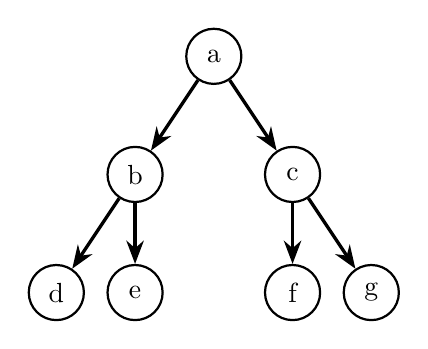
\begin{tikzpicture}[scale=0.5]
                \begin{scope}[every node/.style={circle,thick,draw,minimum size=\nodesize}]
                    \node (a) at (0,6) {a};
                    \node (c) at (2,3) {c};
                    \node (b) at (-2,3) {b};
                    \node (d) at (-4,0) {d};
                    \node (e) at (-2,0) {e};
                    \node (f) at (2,0) {f};
                    \node (g) at (4,0) {g};
                \end{scope}

                \begin{scope}[>={Stealth[black]},
                    every edge/.style={draw=black,very thick}]
                    \path [->] (a) edge node {} (b);
                    \path [->] (a) edge node {} (c);

                    \path [->] (b) edge node {} (d);
                    \path [->] (b) edge node {} (e);

                    \path [->] (c) edge node {} (f);
                    \path [->] (c) edge node {} (g);
                \end{scope}
            \end{tikzpicture}
            \caption{Un albero bilanciato.}
        \end{subfigure}
    \end{figure}
\end{frame}

\begin{frame}\frametitle{Risultati sperimentali II -{}- {\normalsize Paige-Tarjan, Saha}}
    \begin{figure}
        \centering
        \begin{subfigure}{\textwidth}
            \begin{tikzpicture}
                \begin{axis}[
                    axis on top,
                    width=0.98\textwidth,
                    height=4cm,
                    legend style={nodes={scale=0.7, transform shape}, fill=white,opacity=0.8, at={(0,0.67)},anchor=south west, legend columns=1},
                    legend cell align={left},
                    ytick style={draw=none},
                    xtick style={draw=none},
                    xlabel={\footnotesize Numero di nodi},
                    ylabel={\footnotesize Tempo medio (secondi)},
                    xtick={0.0, 500.0, 1000.0, 1500.0, 2000.0},
                    xtick={0, 500, 1000, 1500, 2000},
                    ymode=log,
                    grid=major,
                    title={\footnotesize Aggiornamento della massima bisimulazione dopo l'aggiunta di un arco}
                ]
                \addplot table[x=x,y=y] {../experiments/time/saha/random/mean_0_0.txt};
                \addlegendentry{Paige-Tarjan}
                %\addplot table[x=x,y=y] {../experiments/time/saha/random/mean_0_1.txt};
                %\addlegendentry{DPP}
                \addplot table[x=x,y=y] {../experiments/time/saha/random/mean_0_2.txt};
                \addlegendentry{Saha}
                \begin{scope}[on background layer]
                    \draw[pattern color=green,opacity=1,pattern=north west lines] ({rel axis cs:0.885,0.68}) rectangle ({rel axis cs:0.95,0.98});
                \end{scope}
            \end{axis}
            \end{tikzpicture}
        \end{subfigure}

        \bigskip

        \begin{subfigure}{\textwidth}
            \begin{tikzpicture}
                \begin{axis}[
                    axis on top,
                    ybar,
                    bar width=3pt,
                    width=\textwidth,
                    legend cell align={left},
                    legend style={nodes={scale=0.7, transform shape}, fill=white,opacity=0.8, at={(0,0.73)},anchor=south west, legend columns=1},
                    height=5cm,
                    ytick style={draw=none},
                    xtick style={draw=none},
                    enlarge x limits=0.025,
                    enlarge y limits=false,
                    xlabel style={font=\large},
                    ylabel={\footnotesize Secondi},
                    xticklabels={,,}
                ]
                \addplot table[x=x,y=y] {../experiments/time/saha/random/scatter_1_0.txt};
                \addlegendentry{Paige-Tarjan}
                \addplot+[xshift=-0.1cm] table[x=x,y=y] {../experiments/time/saha/random/scatter_1_2.txt};
                \addlegendentry{Saha}
                \begin{scope}[on background layer]
                    \fill[pattern color=green,opacity=1,pattern=north west lines] ({rel axis cs:0.0,0.0}) rectangle ({rel axis cs:1.0,1.0});
                \end{scope}
            \end{axis}
            \end{tikzpicture}
        \end{subfigure}
    \end{figure}
\end{frame}

\begin{frame}\frametitle{Conclusione}
    Il software sviluppato consente di osservare e confrontare il comportamento degli algoritmi su varie tipologie di grafo.

    \bigskip\bigskip

    \textbf{Sviluppi futuri}
    \begin{itemize}
        \item Pubblicazione di \texttt{BisPy} su JOSS (\emph{Journal of Open Source Software});
        \item Ricalcolo incrementale della massima bisimulazione dopo la \textbf{rimozione} di un arco;
        \item Calcolo della massima bisimulazione con \emph{labeled edges};
        \item Integrazione con altre librerie (\texttt{NetworkX});
        \item \texttt{Cython} per parti critiche del codice.
    \end{itemize}
\end{frame}

\begin{frame}{}
    \centering \Large
    \underline{\emph{Grazie per l'attenzione}}
  \end{frame}

  \begin{frame}\frametitle{Risultati sperimentali III -{}- {\normalsize Paige-Tarjan, Saha}}
    \centering
    \begin{figure}[b!]
        \centering
        \begin{subfigure}[t]{0.48\textwidth}
            \begin{tikzpicture}
                \begin{axis}[
                    axis on top,
                    width=\textwidth,
                    ytick style={draw=none},
                    xtick style={draw=none},
                    legend style={fill=white,opacity=0.8, at={(0,0.68)},anchor=south west, legend columns=1},
                    legend cell align={left},
                    xlabel={Profondità dell'albero},
                    xlabel style={font=\large},
                    ylabel={Secondi},
                    ylabel style={font=\large},
                    xtick={5.0,6.0,7.0,8.0,9.0,10.0},
                    xticklabels={5,6,7,8,9,10},
                    ymode=log,
                    grid=major,
                    title={Alberi bilanciati}
                ]
                \addplot table[x=x,y=y] {../experiments/time/saha/tree/first/mean_0_0.txt};
                \addlegendentry{Paige-Tarjan}
                %\addplot table[x=x,y=y] {experiments/time/saha/tree/first/mean_0_1.txt};
                %\addlegendentry{DPP}
                \addplot table[x=x,y=y] {../experiments/time/saha/tree/first/mean_0_2.txt};
                \addlegendentry{Saha}
            \end{axis}
            \end{tikzpicture}
        \end{subfigure}
        \hfill
        \begin{subfigure}[t]{0.48\textwidth}
            \begin{tikzpicture}
                \begin{axis}[
                    axis on top,
                    width=\textwidth,
                    legend style={fill=white,opacity=0.8, at={(0,0.41)},anchor=south west, legend columns=1},
                    legend cell align={left},
                    xlabel={Profondità dell'albero},
                    xlabel style={font=\large},
                    ylabel style={font=\large},
                    yminorticks=false,
                    xtick={5.0,6.0,7.0,8.0,9.0,10.0},
                    xticklabels={5,6,7,8,9,10},
                    ymode=log,
                    grid=major,
                    title={Raggruppamento per tipo di arco}
                ]
                \addplot table[x=x,y=y] {../experiments/time/saha/tree/first/mean_0_0.txt};
                \addlegendentry{Paige-Tarjan}
                %\addplot table[x=x,y=y] {experiments/time/saha/tree/first/mean_0_1.txt};
                %\addplot table[x=x,y=y] {experiments/time/saha/tree/second/data1.txt};
                %\addplot table[x=x,y=y] {experiments/time/saha/tree/second/data2.txt};
                \addplot table[x=x,y=y] {../experiments/time/saha/tree/second/data3.txt};
                \addlegendentry{Saha $\Delta v = \hphantom{-}3$}
                \addplot table[x=x,y=y] {../experiments/time/saha/tree/second/datam0.txt};
                \addlegendentry{Saha $\Delta v = \hphantom{-}0$}
                \addplot table[x=x,y=y] {../experiments/time/saha/tree/second/datam1.txt};
                \addlegendentry{Saha $\Delta v = -1$}
                %\addplot table[x=x,y=y] {experiments/time/saha/tree/second/datam2.txt};
                %\addplot table[x=x,y=y] {experiments/time/saha/tree/second/datam3.txt};
                %\addplot table[x=x,y=y] {experiments/time/saha/tree/second/datam4.txt};
                %\addlegendentry{Saha $\Delta v = -4$}
            \end{axis}
            \end{tikzpicture}
        \end{subfigure}
    \end{figure}
\end{frame}

\end{document}
